\documentclass[a4paper]{article}
\usepackage{graphicx}
\usepackage{listings}
\usepackage{rotating}
\usepackage{subcaption}
\usepackage[export]{adjustbox}
\usepackage{hyperref}
\usepackage{amsmath}
\usepackage{cite}
%\usepackage[margin=2in]{geometry}
\begin{document}
\lstset{basicstyle=\ttfamily\footnotesize, breaklines=true}
\centerline{\Large \bf An Investigative Framework for Automatic Hardware Generation}
\medskip
\centerline{\bf Alexander Lown}
\bigskip

\begin{abstract}
  A feasibility study is conducted into automatically generating hardware for a binary program, allowing offloading of program critical regions to an adjacent configurable logic block for a host processor.
  A program is created that demonstrates a heuristic-based technique for analysing and transliterating conventional ARM programs into a HDL, without access to the original source code, albeit with a non-trivial set of restrictions in the demonstrated implementation.
\end{abstract}

%------------------------------------------------------------------------------
\section{Introduction}
I investigated the ability to automatically speed-up (or reduce power of) parts of existing applications, without a need to write custom offload hardware for each program, or even to re-compile; in a computing system with both conventional CPUs but also some configurable logic (FPGA fabric-like) area, which I will refer to as an \emph{FPGA-soc}.

For readers unfamiliar with FPGA, these can be thought of as a large quantity of user-configurable logic gates, capable of evaluating extensive logical expressions at high speed (hundrends of megahertz). Ordinarily such logic performs 'calculations' immediately (ignoring propogation delays), but by synchronising work to a clock signal, and through constructions such as finite state machines, it is possible to emulate sequential 'instructions' in a manner equivalant to a Turing machine processing a tape, which is the basis of models used for programming conventional computer processors.

The intention of this work is to take calculations that take a long time to process on a conventional process, and perform as much work in parallel as possible through converting the representation to a set of logical expressions ideal for running on the FPGA. Whilst this is something that is done by humans at the moment, this work intends to demonstrate a method of automating such work, enabling programs to run faster without needing extensive human-performed optimization to utilise the FPGA.

One such example of a computing system are the Xilinx Zynq series ICs, of which I have been working using a Zynq ZC702\cite{ZC702} development board, which contains a xc7z020 IC at its core. The xc7z020 IC contains a dual core ARM Cortex A9 'processor' (hereafter referred to as the PS) along with full MMU, DDR3 controller and APB peripherals (UART, Ethernet, SD, etc.), as well as a large programmable logic area based off a 28nm HKMG fabrication (hereafter referred to as the PL). A variety of AXI ports (and assosciated control signals such as user configurable clocks and interrupts) enabling communication between the PS and PL at high speed. Refer to figure \ref{fig:inter-block} for a detailed overview of how the PS and PL are interconnected. Whilst this is a quite specific system, there are strong parallels with a more conventional (as of the 2000s-2015s) PC, which could be supplemented with a PL card over PCI-E, in the same way that graphics tasks are offloaded to custom silicon in the form of a dedicated GPU, or more recent processing assistance designs such as the Xeon Phi.

This project uses the High Performance AXI controllers connected to some soft-IP performing DMA to enable the PL to interact directly with user-memory whilst running. Programs are run on top of Linux on the PS, rather than working only with bare metal enabling a significantly increased use-case. A kernel module (XDMA) grants user-space access to this DMA'd memory enabling any program to take advantage of it for offloading.

The project requires the existence of several connected fragments to work: the default HDL implementation, which is extended with HDL generated from analysis of the elf binary run on the PS in userspace (and optionally fed with profiling data to suggest blocks to preferrentially run on the PS, interacting through DMA using the kernel-exposed interface.

The project is designed currently to only work with basic blocks (BBs) which are sequences of instructions without any conditional, branching or jumping behaviour for simplicity. There is no reason it would not be possible to add support for these constructs in further work.

\begin{figure}[p]
  \includegraphics[width=1.4\textwidth,center]{fig/interconnect-block.eps}
  \caption{Xilinx UG585\cite{ug585} Figure 5-1: Interconnect Block Diagram}
  \label{fig:inter-block}
\end{figure}

%------------------------------------------------------------------------------
\section{Background}
  \subsection{Initial State Investigation}

  I investigated the existing behaviour of the Zynq ZC702 development board using a variety of metrics in several situations, which will prove useful for Phases 2 and 3.
  This report will present an overview of the collected data, and will draw some conclusion for baseline behaviour.\\
  I have used 2 different benchmarks - the VTR 'basic' regression tests, and the encoding of a 10 second clip of 1280x720 resolution video (from Sintel) from YUV (y4m variant) to h264 using the x264 project.
  The choice of this second benchmark is related to one of the 'proposed' end-cases for this research project - namely hardware offloading of video encoding without the need for the encoder to be specifically written to target the Zynq PL.\\
  The collected data includes runtime, power, current, voltage and temperature information from the on-board PMICs, as well as system memory usage. The PS supports 3 speed steps (222MHz, 333MHz and 667MHz), but due to limitations of the peripheral clocks, only the latter two steps are valid states for testing.

\subsubsection{VTR}
  \paragraph{Runtime}
    Table \ref{tab:vtr:rt} shows the runtime for the various PS clock speeds.
    \begin{table}[tbp]
      \centering
      \begin{tabular}{l | l}
        Speed/MHz & Runtime/s \\
        \hline
        333 & 645 \\
        667 & 343 \\
      \end{tabular}
      \caption{Runtime vs Speed of PS for VTR}
      \label{tab:vtr:rt}
    \end{table}
    This suggests that halving the clock speed does not quite double the actual runtime. I propose that this is due to a reduction in the number of clocks spent idling on memory accesses, resulting in a more efficent usage of each clock cycle.

  \paragraph{Power}
    Figures \ref{fig:vtr:pow:667} and \ref{fig:vtr:pow:333} shows the 'power' as reported by the onboard PMIC for the VCCPx rails (power the PS) and VCCADJ rail (powers the DDR3 memory ICs and the corresponding IO banks).
    \begin{figure}[p]
      \includegraphics[width=\textwidth]{data/fig/vtr:pow:667.eps}
      \caption{Power usage of VTR at 667MHz}
      \label{fig:vtr:pow:667}
    \end{figure}
    \begin{figure}[p]
      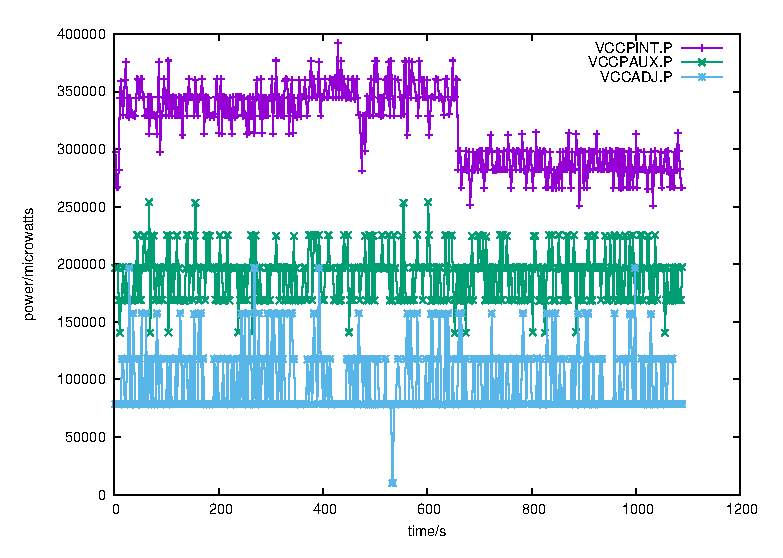
\includegraphics[width=\textwidth]{data/fig/vtr:pow:333.eps}
      \caption{Power usage of VTR at 333MHz}
      \label{fig:vtr:pow:333}
    \end{figure}
    There is a clear uptick in VCCPINT usage after the first 4 samples, which is when the test is started. There is a large deviation in VCCPINT draw over the course of the benchmark at 667MHz, but a signifcantly reduced deviation when run at 333MHz - which I propose is due to the fewer stalls of the processor on memory accesses. On the other hand, VCCADJ's power usage at 333MHz is consistently higher, whilst at 667MHz, it peaks briefly but then returns to baseline for a much longer time - a behaviour I suggest follows on from it being able to complete trannsfers in a shorter time at the higher clock rate, enabling it to return the memory bus to idle sooner.

  \paragraph{Memory}
    Figures \ref{fig:vtr:mem:667} and \ref{fig:vtr:mem:333} show system memory usage for active pages, anonymous pages and the total committed address space during the running of the VTR tests.
    \begin{figure}[p]
      \includegraphics[width=\textwidth]{data/fig/vtr:mem:667.eps}
      \caption{Memory usage of VTR at 667MHz}
      \label{fig:vtr:mem:667}
    \end{figure}
    \begin{figure}[p]
      \includegraphics[width=\textwidth]{data/fig/vtr:mem:333.eps}
      \caption{Memory usage of VTR at 333MHz}
      \label{fig:vtr:mem:333}
    \end{figure}
    These show the allocated of anonymous pages for VTR (and its assosciated tools) to run in. The profiles are pretty similar during both sets of tests, due to changing the speed having little effect on the amount of memory needed. The major spikes in committed address space correspond directly to sudden decreases in the number of active pages - possibly an effect of the deallocations having occurred but the address space not being marked as uncommitted until after the next set of allocations has occurred.

\subsubsection{x264}
  \paragraph{Runtime}
    Table \ref{tab:x264:rt} shows the runtime for the various PS clock speeds.
    \begin{table}[tbp]
      \centering
      \begin{tabular}{l | l}
        Speed/MHz & Runtime/s \\
        \hline
        333 & 122 \\
        667 & 62 \\
      \end{tabular}
      \caption{Runtime vs Speed of PS for x264 encoding}
      \label{tab:x264:rt}
    \end{table}
    Unlike the VTR benchmarks, the runtime is unaffected by the speed of the processor core, despite making heaving usage of NEON optimizations, the limitation is clearly elsewhere\ldots

  \paragraph{Power}
    Figures \ref{fig:x264:pow:667} and \ref{fig:x264:pow:333} shows the 'power' as reported by the PMIC for the VCCPx rails and VCCADJ rail.
    \begin{figure}[p]
      \includegraphics[width=\textwidth]{data/fig/x264:pow:667.eps}
      \caption{Power usage of x264 at 667MHz}
      \label{fig:x264:pow:667}
    \end{figure}
    \begin{figure}[p]
      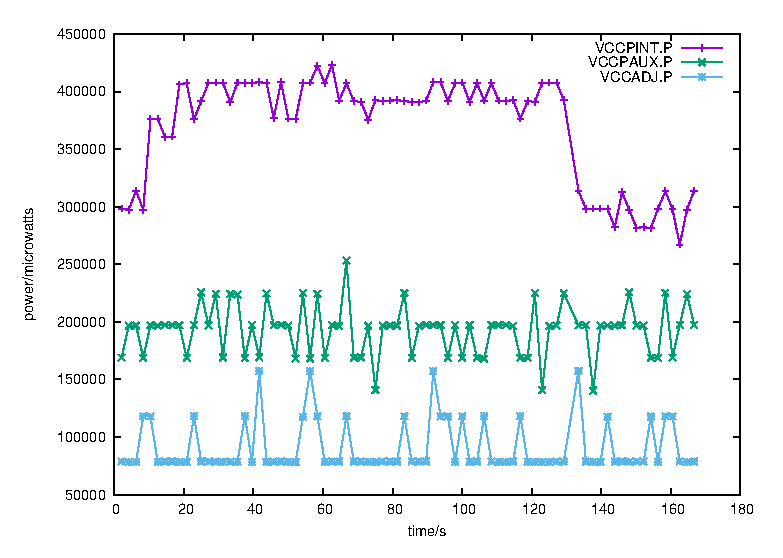
\includegraphics[width=\textwidth]{data/fig/x264:pow:333.eps}
      \caption{Power usage of x264 at 333MHz}
      \label{fig:x264:pow:333}
    \end{figure}
    At 667MHz, there is an increase of 250mW on VCCPINT for the ~62 seconds, but for 333MHz, there is an increase of only 120mW for the 122 seconds, indicating that running at 333MHz consumes less power in total for the same task.

  \paragraph{Memory}
    Figures \ref{fig:x264:mem:667} and \ref{fig:x264:mem:333} show system memory usage.
    \begin{figure}[p]
      \includegraphics[width=\textwidth]{data/fig/x264:mem:667.eps}
      \caption{Memory usage of x264 at 667MHz}
      \label{fig:x264:mem:667}
    \end{figure}
    \begin{figure}[p]
      \includegraphics[width=\textwidth]{data/fig/x264:mem:333.eps}
      \caption{Memory usage of x264 at 333MHz}
      \label{fig:x264:mem:333}
    \end{figure}
    These show a fairly constant memory profile, occupying almost half of the total memory to encode 1280x544p footage.

  \paragraph{Profiling}
    The listings \ref{lst:x264:667} and \ref{lst:x264:333} show the gprof data collected from the benchmarked instances of x264.
    \begin{sidewaysfigure}[p]
      \lstinputlisting[firstline=4, lastline=20]{data/x264/vtr-gmount.out-667-profiled}
      \caption{gprof data for x264 at 667MHz}
      \label{lst:x264:667}
    \end{sidewaysfigure}
    \begin{sidewaysfigure}[p]
      \lstinputlisting[firstline=4, lastline=20]{data/x264/vtr-gmount.out-333-profiled}
      \caption{gprof data for x264 at 333MHz}
      \label{lst:x264:333}
    \end{sidewaysfigure}
    At 667MHz, \verb x264_me_search_ref is the main hotspot - due to lots of stalls on memory accesses, which don't stall at 333MHz - due to the 'reduced' latency the PS sees. At 333MHz, \verb x264_pixel_* routines take up the majority of the time, as these routines are performing lots of arithemtic computation on a few pixels. These look like ideal candidates to offload to the PL. A few of the \verb x264_pixel_* routines are shown in listing \ref{lst:x264:ass} to demonstrate.
    \begin{sidewaysfigure}[bp]
      \centering
      \begin{subfigure}[b]{0.45\textwidth}
        \lstinputlisting[firstline=805, lastline=825]{pixel-a.S}
        \caption{The saturation 8x8 calculations using NEON extensions}
      \end{subfigure}
      \qquad
      \begin{subfigure}[b]{0.45\textwidth}
        \lstinputlisting[firstline=401, lastline=417]{mc-a.S}
        \caption{The average (width 16) calculations using NEON extensions}
      \end{subfigure}
      \caption{ARM Assembly for some of the pixel routines from x264}
      \label{lst:x264:ass}
    \end{sidewaysfigure}

    Further investigation of these results showed that they were not as optimal candidaes for offloading as initially suggested, due to the encoding process at the default levels spending too much time in memory accesses, rather than in pure-computational work. As such the profiling data was re-run with higher quality encoding presets of x264. I chose to try use the presets 'slower', 'very slow' and 'placebo'. An overview of the result can be seen in table \ref{tab:x264:prof-extra} and listings \ref{lst:x264:slower}, \ref{lst:x264:very-slow} and \ref{lst:x264:placebo}.

    \begin{sidewaystable}[tbp]
      \centering
      \begin{tabular}{l | p{12cm} | l | l}
        Profile & Equated Flags & Average FPS & Runtime/s \\
        \hline\\
        slower & --b-adapt 2 --direct auto --me umh --partitions all --rc-lookahead 60 --ref 8 --subme 9 --trellis 2  & 0.55 & 190\\
        very-slow & --b-adapt 2 --bframes 8 --direct auto --me umh --merange 24 --partitions all --ref 16 --subme 10 --trellis 2 --rc-lookahead 60 & 0.30  & 347\\
        placebo & --bframes 16 --b-adapt 2 --direct auto --slow-firstpass --no-fast-pskip --me tesa --merange 24 --partitions all --rc-lookahead 60 --ref 16 --subme 11 --trellis 2  & 0.06 & 1733 \\
      \end{tabular}
      \caption{Runtime and Flags for more difficult x264 settings}
      \label{tab:x264:prof-extra}
    \end{sidewaystable}

    \begin{sidewaysfigure}[p]
      \lstinputlisting[firstline=4,lastline=20]{data/x264/x264-slower.gprof}
      \caption{gprof data for x264 using 'slower'}
      \label{lst:x264:slower}
    \end{sidewaysfigure}
    \begin{sidewaysfigure}[p]
      \lstinputlisting[firstline=4,lastline=20]{data/x264/x264-very-slow.gprof}
      \caption{gprof data for x264 using 'very-slow'}
      \label{lst:x264:very-slow}
    \end{sidewaysfigure}
    \begin{sidewaysfigure}[p]
      \lstinputlisting[firstline=4,lastline=20]{data/x264/x264-placebo.gprof}
      \caption{gprof data for x264 using 'placebo'}
      \label{lst:x264:placebo}
    \end{sidewaysfigure}

    These show quite a different picture to the default profile, we can see a large quantity of PS time (and power) being spent in functions such as \verb x264_pixel_ads{14} which are almost entirely arithmetic, along with the NEON optimized \verb x264_pxel_sad_x3_*_neon functions. This suggests that x264 is definitely still a good use case for which PL-backed offloading could result in increased performance, as opposed to simply power reduction.

%------------------------------------------------------------------------------
\section{Completed Work}
Due to the large area of interaction required to make this project complete, there has been work on programs in Linux user space, Linux kernel space, and HDLs (VHDL, Verilog and IP block design), utilizing a variety of tools and languages.

I could include large quantities of this as part of the report, but will chose instead to include only small snippets and point the reader to the Github repositories if they are interested in the full code bases, with all the supporting scripts and build systems - though I warn them that there is ~20-30GB of both proprietary and free tools required to recreate results on hardware. The analysis program by itself, however, runs just fine in any modern Ruby environment and demonstrates the majority of the principles needing no external tools.

The relevant code bases can be found at \url{https://github.com/alown/zynq}, \url{https://github.com/alown/zynq-xdma} and \url{https://github.com/alown/vtr}.

Important information relating to the implementation details can often be found in a \emph{NOTES} file at the root of the repositories.

\subsection{Analysis Program}

In the zynq repository, the analysis program can be found in \verb elf/analysis/* which is a program written in Ruby to take a given ARM ELF binary (in \texttt{objdump -d} form), and optionally a \texttt{GNU Gprof} profiling output to guide the analysis towards known areas of high contention.

It consists of a variety of \emph{phases}, which can be stacked by the user as appropriate, though a conventional call would use something along the lines of the following set, where \emph{phases} are seperated by colons: \texttt{Read:BB:Arith:Loop:GenVHDL}.

I shall now provide a brief description of what each \emph{phase} does.

\subsubsection{\texttt{Read}}

This takes in and 'parses' the \texttt{objdump} file, creating a list of labelled blocks, called here \emph{functions}. For each \emph{function} it parses in the address, instruction and any arguments storing into an in-memory hash.

Optionally, if specified, it will also take the \texttt{gprof} file, parsing it similarly into a hash of \emph{functions} to profile data such as percentage of total runtime, or number of calls.

\subsubsection{\texttt{BB}}

Simply iterates through each \emph{function}, breaking it down it \emph{basic-blocks} (\emph{BBvs}), which are denominated here by a branch/jump instruction. It also attaches any profiling data to the basic block.

\subsubsection{\texttt{Arith}}

Iterates through all the \emph{BBs} looking for arithmetic instructions, recording the quantity and length of uninterrupted sequential runs of such instructions, as these are likely to be prime candidates for 'fusing' into an emulated 'single instruction' run on the PL.

\subsubsection{\text{SIMD}}

Performs the same work as \texttt{Arith}, but is records such statistics for SIMD (here: NEON) instructions. As these are only likely to be used in code at already optimized sections, which are likely to correlate with areas of extensive runtime.

\subsubsection{\text{Loop}}

Scans all the \emph{BBs} for subsections where the control flow seems to loop - here taken to be a branch/jump instruction to an location behind the PC. After finding such a subsection, it then attempts to determine key factors of the known loop styles which would enable efficent transliteration of them.
Support here only extends to simple C-style for loops, as the \texttt{GCC} compiler tends to produce these in a easy-to-find form: Counter initialization, an arithmetic operation on the counter variable, a compare condition for loop termination, the loop body's work, and finally the looping branch instruction.
This leaves open the option to use the following heuristic for such style loops, see figure \ref{fig:loop-method}.

\begin{enumerate}
  \item Work backwards from the suspicious branch instruction to find a relevant compare condition, noting which registers are tested
  \item Work forwards from the start of the loop (as determined by the branch target), looking for an arithmetic operation acting on one of the registers used in the found compare instructions. In this implementation the arithmetic operation should have an immediate operand (a constant change)
    \begin{itemize}
      \item If anything else acts on this now determined loop counter register, then this must be a more complex operation not currently supported
    \end{itemize}
  \item Having determined the loop counter register, we can find where it is written to before the start of the loop, and hence the counter initialization sequence
  \item Any remaming instructions between the branch and the start of the loop, must be the loop body
\end{enumerate}

\subsubsection{\text{GenVHDL}}

Transliterates any 'important enough' \emph{BBs}, and any fully identified loops, and attempts to transliterate them into VHDL using the following algorithm:

\begin{description}
  \item[Firstly] \hfill\\
    'Parallelization' is performed on the \emph{BB}, which iterates through the instructions recording data-flow to enable the production of a data-flow graph.
    Once a data-flow graph is determined, it is possible to 'pull apart' this set of instructions into multiple sets of instructions which can be performed at the same time without interferring with each other as they utilize completely independent register sets. These are referred to as \emph{pars}.
  \item[Transliteration] \hfill\\
    Each \emph{par} can then be iterated over in order and every instruction transliterated using an (effectively) fancy look-up-table into short sequences of VHDL code. Registers are identified and tracked through each \emph{par}. Any modifications cause the generation of a new variable, and subsequent reads from this register now use this variable rather than the initial value, building up extensive logical expressions, taking only the sum of the propogation delays to evaluate, rather than many instruction cycles.
  \item[Loops] \hfill\\
    Loops capable of being fully identified, can be transliterated as described in figure \ref{fig:loop-method}, by making use of the transliteration subsystem for individual independent lines e.g. counter initialization, and the parallelization subsystem can handle sequences of instructions such as the loop body.
  \item[Output] \hfill\\
    All of this information is currently simply dumped to \texttt{stdout}, and insertion into the corresponding hardware harnesses is left to the reader to perform. For \emph{BBs}, this simply involves inserting the generated logic and signals into the clearly delimited sections in the test harness. For loops this requires more extensive signalling and control logic to be written to interface.
\end{description}

\begin{figure}[pb]
  \centering
  \begin{subfigure}[b]{\textwidth}
    \lstinputlisting[lastline=3]{LOOPMISC}
    \caption{C-style for loop}
  \end{subfigure}
  \begin{subfigure}[b]{\textwidth}
    \lstinputlisting[firstline=4]{LOOPMISC}
    \caption{VHDL format this could transliterate to}
  \end{subfigure}
  \caption{Style of currently supported loop transliteration work}
  \label{fig:loop-method}
\end{figure}

\subsection{Supporting Work}

\verb elf/offload.vhdl  is a simple wrapper entity for the generated VHDL that presents some signals representing the r0-r13 registers. This file is where transliterated \emph{BBs} can be simply copy-pasted from the analysis output into the delimited sections before synthesising.
\verb elf/offload-top.vhdl  presents an AXI4-S (AXI-4 streaming) interface to unpack/pack the starting/end values for r0-r13 for the offload block, as well as coordinating everything using a simple FSM.

The Vivado Project \verb tmp/vivado/[\ldots]simple.xpr  holds together all of the generated offloaded code by linking it to the rest of the system using Xilinx DMA IP over the HP0 AXI port described earlier, and shown in figure \ref{fig:inter-block}. A high-level block diagram showing the interactions between the offloaded code (shown as the \verb addtest  IP block), and the rest of the design can be found in figure \ref{fig:vivado-block}.

\begin{sidewaysfigure}
  \centering
  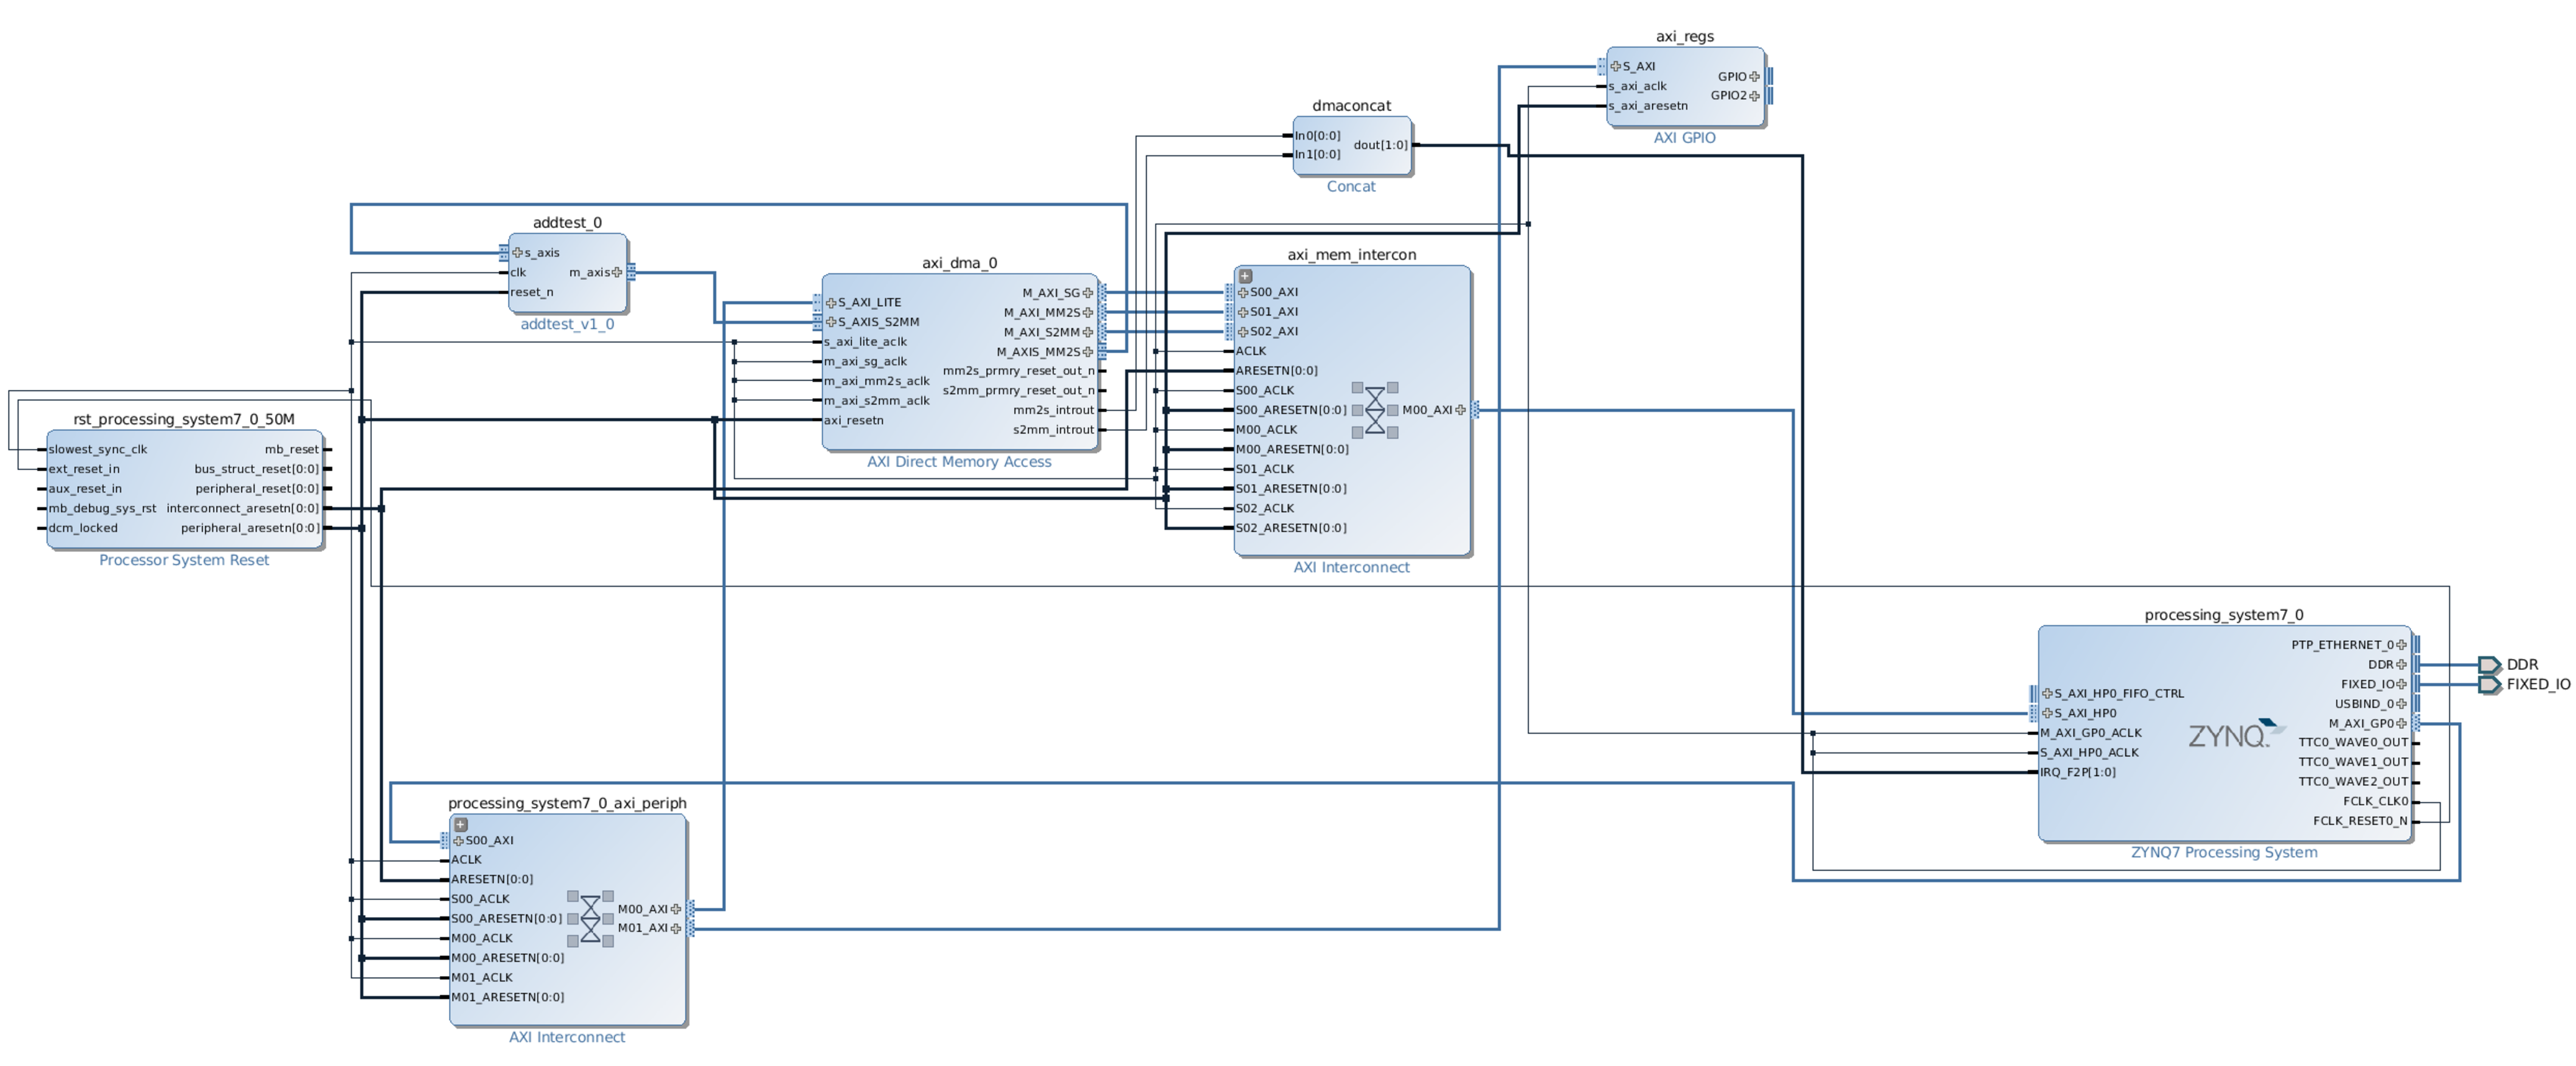
\includegraphics[width=\textwidth]{fig/vivado-block.eps}
  \caption{Vivado Block Design}
  \label{fig:vivado-block}
\end{sidewaysfigure}

\subsection{DMA}

To avoid spending unnecessary time writing and debugging a Linux kernel module to do DMA, I have chosen to extend from an existing project called XDMA, which presents the DMA IP as a block device at \verb /dev/xdma . The XDMA project also came with a simple user-space shared library to make adding support to a new application as easy as linking to the shared library and the transfer function at appropriate times.

I verified the functionality of the PL DMA IP, and the whole userspace stack by originally connected the design with a 1024 deep FIFO over the AXI4-S interface, which then let me perform simple write/wait/read tests from userspace to verify a lack of corruption and to get an idea of the speed of such transfers.
A DMA transfer to/from the FIFO of a $32\text{bit} * 1024 = 4096\text{bytes}$ was able to achieve speeds of ~$190\text{MB/s}$ using an in-PL clock of $150\text{MHz}$.

\verb demo/xdma-offload.c  is a small user-space testing program which performs the required packetization of some possible register values, then transfers to the PL to do work, then reads the resulting register values back out of the DMA engine and prints it back to the user for verification.


\subsection{Initial Hardware Results}

  Together the analysis script when fed in a objdump disassembly (to avoid the need to internally handle disassembly the ELF binary format, keeping the complexity of the analysis system lower) and a gprof profiling file to enable location of program critical sections for offloading, the analysis system is able to parse in BBs, detect sequences of arithmetic instructions (support for NEON arithmetic instructions is included), choose some important sections, and then transliterate into VHDL for a certain limited susbset of arithmetic instructions. (ADD, SUB, MOV, MUL in register-register modes). This generated code can then be included in the hardware framework and then synthesised for an appropriate target device. The host program can then be 'modified' (currently manually) to do the appropriate DMA transfers to/from the hardware framework. This enables demonstration of offloading of very simple programs to hardware, allowing us to benchwark the situation. Refer to table \ref{table:offload-simple} for results.

  \begin{table}[btp]
    \centering
    \begin{tabular}{l|l}
      Mode & Runtime/$\mu S$\\
      \hline\\
      Host CPU only & 1 \\
      Offloaded using DMA & 60
    \end{tabular}
    \caption{Offloading results for a fused 10-deep integer mul-add sequence including DMA transfer time (arm-test/ma.c )}
    \label{table:offload-simple}
  \end{table}

\subsection{Analysis Demonstrations}

Having now covered the fundamentals, I shall provide a few simple demonstrations of the analysis system.

\subsubsection{Instruction Fusing 1}
Refer to figure \ref{fig:if1}.
This illustrates analysis of a very simple set of chained addition instructions, demonstrating the possibility for performing automated instruction fusing.

\begin{sidewaysfigure}[hp]
  \begin{subfigure}[b]{0.5\textwidth}
    \lstinputlisting[firstline=3,lastline=6]{ex/tools/trans_dp.c}
    \lstinputlisting[firstline=7,lastline=11]{ex/tools/trans_dp.dis}
    \caption{C form of function and Disassembly}
  \end{subfigure}
  \begin{subfigure}[b]{0.5\textwidth}
    \lstinputlisting[firstline=93,lastline=109]{ex/tools/trans_dp.anal}
    \caption{Transliterated output}
  \end{subfigure}
  \caption{Simple chained addition}
  \label{fig:if1}
\end{sidewaysfigure}

\subsubsection{Instruction Fusing 2}
Refer to figure \ref{fig:if2}.
This illustrates analysis of a compiler unrolled loop perfroming a multiply-add instruction repeatedly to some data in registers.
As it is fully unrolled, the analysis is able to perform extended instruction fusing for this sequence, allowing (at the expense of a non-trivial amount of logic cells) a sequence of 10 32-bit multiplies and 32-bit additions in sequence, in only the time of the propogation through this tree on PL.

\begin{sidewaysfigure}[hp]
  \begin{subfigure}[b]{0.5\textwidth}
    \lstinputlisting[firstline=1,lastline=7]{ex/possibilites/loops.c}
    \lstinputlisting[firstline=7,lastline=17]{ex/possibilites/loops.dis}
    \caption{C form of function and Disassembly}
  \end{subfigure}
  \begin{subfigure}[b]{0.5\textwidth}
    \lstinputlisting[firstline=617,lastline=646]{ex/possibilites/loops.anal}
    \caption{Transliterated output}
  \end{subfigure}
  \caption{Compiler unrolled loop, results in extensive fusing}
  \label{fig:if2}
\end{sidewaysfigure}

\subsubsection{Loops - partially unrolled by nesting}
Refer to figure \ref{fig:loop-partial}.
This illustrates analysis of a fairly common nested loop scenario, but which the analysis program is able to fully identify allowing direct transliteration into a logic process, whilst still performing the inner loop in only the propogation time. This example demonstrates the most complicated instruction sequence the analysis program is currently able to fully handle.

\begin{sidewaysfigure}[hp]
  \begin{subfigure}[b]{0.5\textwidth}
    \lstinputlisting[firstline=26,lastline=33]{ex/possibilites/loops.c}
    \lstinputlisting[firstline=38,lastline=51]{ex/possibilites/loops.dis}
    \caption{C form of function and Disassembly}
  \end{subfigure}
  \begin{subfigure}[b]{0.5\textwidth}
    \lstinputlisting[firstline=2116,lastline=2140]{ex/possibilites/loops.anal}
    \caption{Transliterated output}
  \end{subfigure}
  \caption{Nested loop, partially unrolled}
  \label{fig:loop-partial}
\end{sidewaysfigure}

\section{Evalution}
\subsection{Problems Left}
The transliteration generates VHDL, because of personal preference (and the much stricter types make keeping the distinctions between signed and unsigned operations more visible). To enable this work to be joined up with the open-toolchain that was originally intended (a VTR-backed) flow, this would need to be changed to generate Verilog instead due to synthesis limitations.

Support for significantly more instructions in the transliteration phase would make this work much more applicable to a real-world situation. The original intention was to demonstrate offloading of a critical section of x264 video encoder, but support was never completed, due to the necessity to be able to handle memory-backed data - necessitating a need to understand load and store instructions.

Support for loading from memory and storing to memory, would remove the basic-block limitation that this work has been hindered by - as most real-work programs make extensive use, and even calculation heavy programs such as x264 continue to do large quantities of memory usage during critical loops. The Zynq platform theoretically enables support for this, through the use of the cache-coherency port, whilst the Linux host will take care of any access to pages that are not currently resident in pages if required. This would increase the complexity of the hardware framework fairly significantly however, as it requires either stalling the offload-pipeline or re-implementing a fair amount of any processors load/store coherency system, with forwarding lines to enable performance to be kept at a reasonable level.

Hardware limitations mostly resolve around the very high latency to offload any program, due to the large quantity of information needed to be transferred, and the relatively small size of the AXI ports available between the system. Even something as simple as a few registers (when 32-bits each) requires a clock per register/register-pair (if using the ports in 64-bit mode). By the time a DMA transfer has been scheduled in the kernel for each direction, and then completed, the latency is sufficently large to be restrictive (on the order of thousands of CPU clocks at 600MHz). Alternative silicon designs with larger CPU-Hardware interfaces (in the same way CPU-Memory interfaces have consistently increased in size) would alleviate these problems.

\section{Scope for Future Works}
\subsection{Other Works}
Existing attempts at offloading programs such as Xilinx Vivado HLS\cite{hls}, and Maxeler\cite{mf-fpga} Java interfaces both present their own limitations in this field.

Vivado HLS requires extra information over a standard C program to enable efficent offloading, and has resulted in an incompatible C-like language, thereby removing the advantages (of relocation) that writing in C offers.

Maxela requires a completely custom Java program to be written tailored for your end use case, that utilises a variety of Maexla specific types and bindings, completely removing the advantage of a high level language, and requiring the programmer to think about when and how they wish to offload specific sections of code.

Other works can be found in the GPU space, with the recent advances in general purpose computing on previously graphics specific devices, with toolchains based around working with CUDA\cite{cuda} or OpenCL. Once again though, these required either writing your own kernel, or accepting a variety of limitations in a higher level language that is converted.

\subsection{Recommendations for future works}
I would recommend that future works based on the same (or very similar) hardware systems to the Zynq XC7Z0* silicon choose to focus on offloading loops using a pipelined hardware framework to hide the latency issues on the system. Memory loads/stores could be handlede through either the CCP, or through careful handling in hardware, and then transferring and batching back onto the CPU.

Ideally future users would have input into the SOC design enabling a higher bandwidth interface to be specified between the logic and the host CPU, enabling latency problems to be removed. If sufficent control over the host CPU core is available, then it would be possible to allow for reserved instruction space to be used to trigger offloading, without needing to schedule for a peripheral transfer from the host OS.

\section{References}
\bibliographystyle{plain}
\bibliography{phase3}

\end{document}
